% Manuscript-ready consensus-sensitivity section.
% Numeric results are generated only after the strict three-session evidence gate.
% Requires: booktabs, adjustbox, tikz, pgfplots; \pgfplotsset{compat=1.18}

\subsection{Consensus-Layer Sensitivity: PoS versus Roll-DPoS}
\label{sec:pos-rolldpos-method}

The consensus mechanism is a property of the execution network rather than of the
Solidity contract. We therefore evaluate consensus-layer sensitivity by deploying
the identical \texttt{Stage3AnomalyLedger} creation bytecode to two EVM-compatible
public testnets: Ethereum Sepolia and IoTeX testnet. Sepolia follows the Ethereum
PoS protocol but uses a permissioned validator set operated by client and testing
teams \cite{ethereumNetworks}; this restriction is stated explicitly to avoid
generalising testnet behaviour to Ethereum mainnet. IoTeX documents its consensus
as Randomized Delegated Proof of Stake (Roll-DPoS), which combines delegated
candidate election, VRF-based committee selection, and PBFT voting
\cite{iotexRollDpos}. IoTeX testnet uses chain ID 4690 and exposes an
Ethereum-compatible JSON-RPC interface \cite{iotexTestnet}.

The study uses a paired concurrent-submission design. In each session, both
contracts receive three excluded warm-up pairs followed by $R=30$ measured pairs.
A pair carries the same commitment and evidence digest on both networks, and the
two transactions are submitted concurrently from the same client host. We collect
at least three sessions in separate time windows ($N\geq90$ matched pairs), while
holding the client host, RPC provider per network, compiler configuration, contract
bytecode, fixed transaction gas limit, and confirmation rule constant. Runtime-code
Keccak-256 hashes are checked after every deployment. The primary metric is the
client-observed interval from transaction submission to first successful receipt.
It includes RPC/client overhead and prevailing public-testnet load and is therefore
reported as \emph{first-inclusion latency}, not economic-finality latency.

For each network, the harness additionally records deployment and anchor gas,
effective gas price, block identifiers and timestamps, and at least 64 consecutive
post-run block headers. Duplicate-commitment, zero-commitment, and unauthorised-
submitter rejections are exercised as read-only \texttt{eth\_call} probes against
the deployed state. Gas prices are retained for provenance but are not converted
into a cross-asset cost comparison. Medians, quartiles, P95, means, and sample
standard deviations are derived from raw JSON evidence. Median confidence intervals
use a deterministic two-level hierarchical bootstrap that resamples sessions and
then matched pairs within sessions (10,000 replicates). The analysis fails closed
when a chain ID, bytecode hash, receipt, event, security probe, session count, or
repetition count is incomplete.

\subsection{Consensus-Layer Sensitivity Results}
\label{sec:pos-rolldpos-results}

% These files do not exist until measured evidence from both networks passes the
% publication gate. Their absence prevents unmeasured numbers from entering the paper.
\IfFileExists{derived_consensus/results_pos_rolldpos.tex}{%
  % AUTO-GENERATED from measured benchmark.json evidence; do not hand-edit.
Across 90 matched transaction pairs collected in 3 independent sessions, median client-observed first-inclusion latency was 12426.58~ms on Ethereum Sepolia and 7225.15~ms on IoTeX testnet (Table~\ref{tab:pos-rolldpos}). The median paired difference (Sepolia minus IoTeX) was 4381.82~ms (descriptive hierarchical-bootstrap 95\% interval: 3930.60--7909.77~ms), and the median paired Sepolia-to-IoTeX latency ratio was 1.87 (descriptive hierarchical-bootstrap 95\% interval: 1.48--2.74). With only three session clusters, these intervals summarise the retained sessions and are not claimed to have reliable nominal frequentist coverage. The median anchor execution gas was 48973 and 43685, respectively. Identical runtime bytecode and calldata do not force equal gas across different EVM-compatible chains because execution rules are chain-configured; the retained evidence has no opcode traces, so the difference is reported descriptively rather than assigned to a particular fork. Gas-price values are not converted into a cross-asset economic comparison. All three read-only rejection probes (duplicate, zero, and unauthorised submitter) reverted on both deployed contracts. These values describe public-testnet first inclusion for the isolated audit-anchor transaction and do not imply mainnet finality or production O-RAN performance.

  % AUTO-GENERATED from measured benchmark.json evidence; do not hand-edit.
\begin{table*}[!t]
\centering
\caption{Paired public-testnet consensus sensitivity of the identical Stage3AnomalyLedger bytecode. Latency is client-observed submission to first inclusion, not economic finality; brackets are hierarchical-bootstrap 95\% confidence intervals for the median.}
\label{tab:pos-rolldpos}
\begin{adjustbox}{width=\textwidth}
\begin{tabular}{lrrrrrr}
\toprule
Network (consensus) & Chain ID & Anchor gas & Median latency (ms) & P95 latency (ms) & Block interval (s) & Rejections \\ 
\midrule
Ethereum Sepolia (Gasper PoS) & 11155111 & 48973 & 12426.58 [12394.75, 12455.95] & 24614.54 & 12.00 & 3/3 \\
IoTeX testnet (Roll-DPoS) & 4690 & 43685 & 7225.15 [4538.58, 8493.93] & 8763.75 & 3.00 & 3/3 \\
\bottomrule
\end{tabular}
\end{adjustbox}
\end{table*}

  % AUTO-GENERATED from measured benchmark.json evidence; do not hand-edit.
\begin{figure}[!t]
\centering
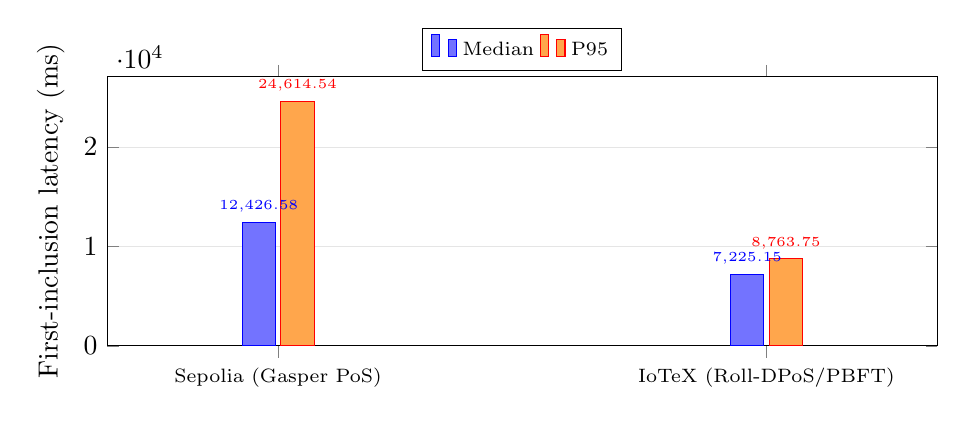
\begin{tikzpicture}
\begin{axis}[
  width=\columnwidth,height=5.0cm,ybar,bar width=12pt,
  ylabel={First-inclusion latency (ms)},
  symbolic x coords={Sepolia,IoTeX},xtick=data,
  xticklabels={Sepolia (Gasper PoS),IoTeX (Roll-DPoS/PBFT)},
  x tick label style={font=\scriptsize,align=center},
  legend style={at={(0.5,1.02)},anchor=south,legend columns=2,font=\scriptsize},
  ymin=0,nodes near coords,nodes near coords style={font=\tiny},
  enlarge x limits=0.35,ymajorgrids,grid style={black!10}
]
\addplot+[fill=blue!55] coordinates {(Sepolia,12426.58) (IoTeX,7225.15)};
\addplot+[fill=orange!70] coordinates {(Sepolia,24614.54) (IoTeX,8763.75)};
\legend{Median,P95}
\end{axis}
\end{tikzpicture}
\caption{Measured client-observed first-inclusion latency for matched,
concurrently submitted audit-anchor transactions. Public-testnet load and
RPC/client overhead are included; economic finality is not measured. Raft and
QBFT are compared structurally in Fig.~\ref{fig:consensus-protocols} but are
reported separately because their workloads and estimands are not comparable.}
\label{fig:pos-rolldpos-latency}
\end{figure}

}{%
  \emph{No PoS--Roll-DPoS numerical result is claimed in this source snapshot;
  the measured three-session evidence package has not yet been supplied to the
  deterministic analysis gate.}%
}

The comparison is intentionally bounded to a public-testnet audit-anchor
micro-benchmark. It does not estimate mainnet throughput, validator
decentralisation, economic finality, or end-to-end O-RAN performance. In particular,
any latency difference may reflect block cadence, RPC implementation, propagation,
or transient load in addition to the underlying consensus protocol; causal
attribution beyond the measured observables is therefore avoided.
